\section{2. Root and Launch Surface}\label{root-and-launch-surface}

This section maps the top-level files and folders that tell a newcomer
what MCP-Geo is, how to run it, and how the project frames its own
maturity.

\subsection{2.1 First-run orientation and launch
files}\label{first-run-orientation-and-launch-files}

This subsection groups the files that explain the repo fastest to a
first-time operator.

The quickest route into the repository is still the
\href{https://github.com/chris-page-gov/mcp-geo/blob/fe862910da246ca77f374cfbe484985f5df4d316/README.md\#L20-L126}{README
start-here path}, supported by the
\href{https://github.com/chris-page-gov/mcp-geo/blob/fe862910da246ca77f374cfbe484985f5df4d316/Dockerfile}{Dockerfile},
the
\href{https://github.com/chris-page-gov/mcp-geo/blob/fe862910da246ca77f374cfbe484985f5df4d316/.env.example}{environment
template}, the
\href{https://github.com/chris-page-gov/mcp-geo/blob/fe862910da246ca77f374cfbe484985f5df4d316/mcp.json}{runtime
metadata in \texttt{mcp.json}}, and the lightweight
\href{https://github.com/chris-page-gov/mcp-geo/blob/fe862910da246ca77f374cfbe484985f5df4d316/tutorial.md}{tutorial
note}. Read this cluster when the immediate question is ``How do I start
it?'' rather than ``How is it built?''.

Where to go:
\href{https://github.com/chris-page-gov/mcp-geo/blob/fe862910da246ca77f374cfbe484985f5df4d316/README.md\#L1-L240}{README.md},
\href{https://github.com/chris-page-gov/mcp-geo/blob/fe862910da246ca77f374cfbe484985f5df4d316/Dockerfile}{Dockerfile},
\href{https://github.com/chris-page-gov/mcp-geo/blob/fe862910da246ca77f374cfbe484985f5df4d316/.env.example}{\texttt{.env.example}},
\href{https://github.com/chris-page-gov/mcp-geo/blob/fe862910da246ca77f374cfbe484985f5df4d316/mcp.json}{\texttt{mcp.json}},
and
\href{https://github.com/chris-page-gov/mcp-geo/blob/fe862910da246ca77f374cfbe484985f5df4d316/tutorial.md}{tutorial.md}.

\subsection{2.2 Durable context, governance, and contributor
controls}\label{durable-context-governance-and-contributor-controls}

This subsection points to the files that explain how the repo governs
itself while it is being built and reviewed.

The project explains its own limits and working style in a tight
root-level cluster:
\href{https://github.com/chris-page-gov/mcp-geo/blob/fe862910da246ca77f374cfbe484985f5df4d316/AGENTS.md}{AGENTS.md},
\href{https://github.com/chris-page-gov/mcp-geo/blob/fe862910da246ca77f374cfbe484985f5df4d316/CONTEXT.md}{CONTEXT.md},
\href{https://github.com/chris-page-gov/mcp-geo/blob/fe862910da246ca77f374cfbe484985f5df4d316/PROGRESS.MD}{PROGRESS.MD},
\href{https://github.com/chris-page-gov/mcp-geo/blob/fe862910da246ca77f374cfbe484985f5df4d316/CHANGELOG.md}{CHANGELOG.md},
\href{https://github.com/chris-page-gov/mcp-geo/blob/fe862910da246ca77f374cfbe484985f5df4d316/safe-by-design.json}{safe-by-design.json},
\href{https://github.com/chris-page-gov/mcp-geo/blob/fe862910da246ca77f374cfbe484985f5df4d316/documentation.md}{documentation.md},
and
\href{https://github.com/chris-page-gov/mcp-geo/blob/fe862910da246ca77f374cfbe484985f5df4d316/implement.md}{implement.md}.
This is where readers find the repo's durable assumptions, not just its
executable code.

Where to go:
\href{https://github.com/chris-page-gov/mcp-geo/blob/fe862910da246ca77f374cfbe484985f5df4d316/AGENTS.md}{AGENTS.md},
\href{https://github.com/chris-page-gov/mcp-geo/blob/fe862910da246ca77f374cfbe484985f5df4d316/CONTEXT.md}{CONTEXT.md},
\href{https://github.com/chris-page-gov/mcp-geo/blob/fe862910da246ca77f374cfbe484985f5df4d316/PROGRESS.MD}{PROGRESS.MD},
\href{https://github.com/chris-page-gov/mcp-geo/blob/fe862910da246ca77f374cfbe484985f5df4d316/CHANGELOG.md}{CHANGELOG.md},
and
\href{https://github.com/chris-page-gov/mcp-geo/blob/fe862910da246ca77f374cfbe484985f5df4d316/safe-by-design.json}{safe-by-design.json}.

\subsection{2.3 Repository shape at the pinned
commit}\label{repository-shape-at-the-pinned-commit}

This subsection turns the repo root into a readable map by showing which
top-level areas dominate and what each cluster is for.

At the pinned commit, the visible mass of the repository lives in
\href{https://github.com/chris-page-gov/mcp-geo/tree/fe862910da246ca77f374cfbe484985f5df4d316/docs}{docs/},
\href{https://github.com/chris-page-gov/mcp-geo/tree/fe862910da246ca77f374cfbe484985f5df4d316/tests}{tests/},
\href{https://github.com/chris-page-gov/mcp-geo/tree/fe862910da246ca77f374cfbe484985f5df4d316/research}{research/},
\href{https://github.com/chris-page-gov/mcp-geo/tree/fe862910da246ca77f374cfbe484985f5df4d316/scripts}{scripts/},
\href{https://github.com/chris-page-gov/mcp-geo/tree/fe862910da246ca77f374cfbe484985f5df4d316/server}{server/},
\href{https://github.com/chris-page-gov/mcp-geo/tree/fe862910da246ca77f374cfbe484985f5df4d316/tools}{tools/},
\href{https://github.com/chris-page-gov/mcp-geo/tree/fe862910da246ca77f374cfbe484985f5df4d316/playground}{playground/},
and
\href{https://github.com/chris-page-gov/mcp-geo/tree/fe862910da246ca77f374cfbe484985f5df4d316/resources}{resources/}.
That distribution tells the real story of the repo: it is not just a
server, but a working evidence pack around a server.

Where to go:
\href{https://github.com/chris-page-gov/mcp-geo/tree/fe862910da246ca77f374cfbe484985f5df4d316}{repo
root at the pinned commit},
\href{https://github.com/chris-page-gov/mcp-geo/tree/fe862910da246ca77f374cfbe484985f5df4d316/docs}{docs/},
\href{https://github.com/chris-page-gov/mcp-geo/tree/fe862910da246ca77f374cfbe484985f5df4d316/tests}{tests/},
\href{https://github.com/chris-page-gov/mcp-geo/tree/fe862910da246ca77f374cfbe484985f5df4d316/research}{research/},
\href{https://github.com/chris-page-gov/mcp-geo/tree/fe862910da246ca77f374cfbe484985f5df4d316/scripts}{scripts/},
and
\href{https://github.com/chris-page-gov/mcp-geo/tree/fe862910da246ca77f374cfbe484985f5df4d316/server}{server/}.

\begin{figure}
\centering
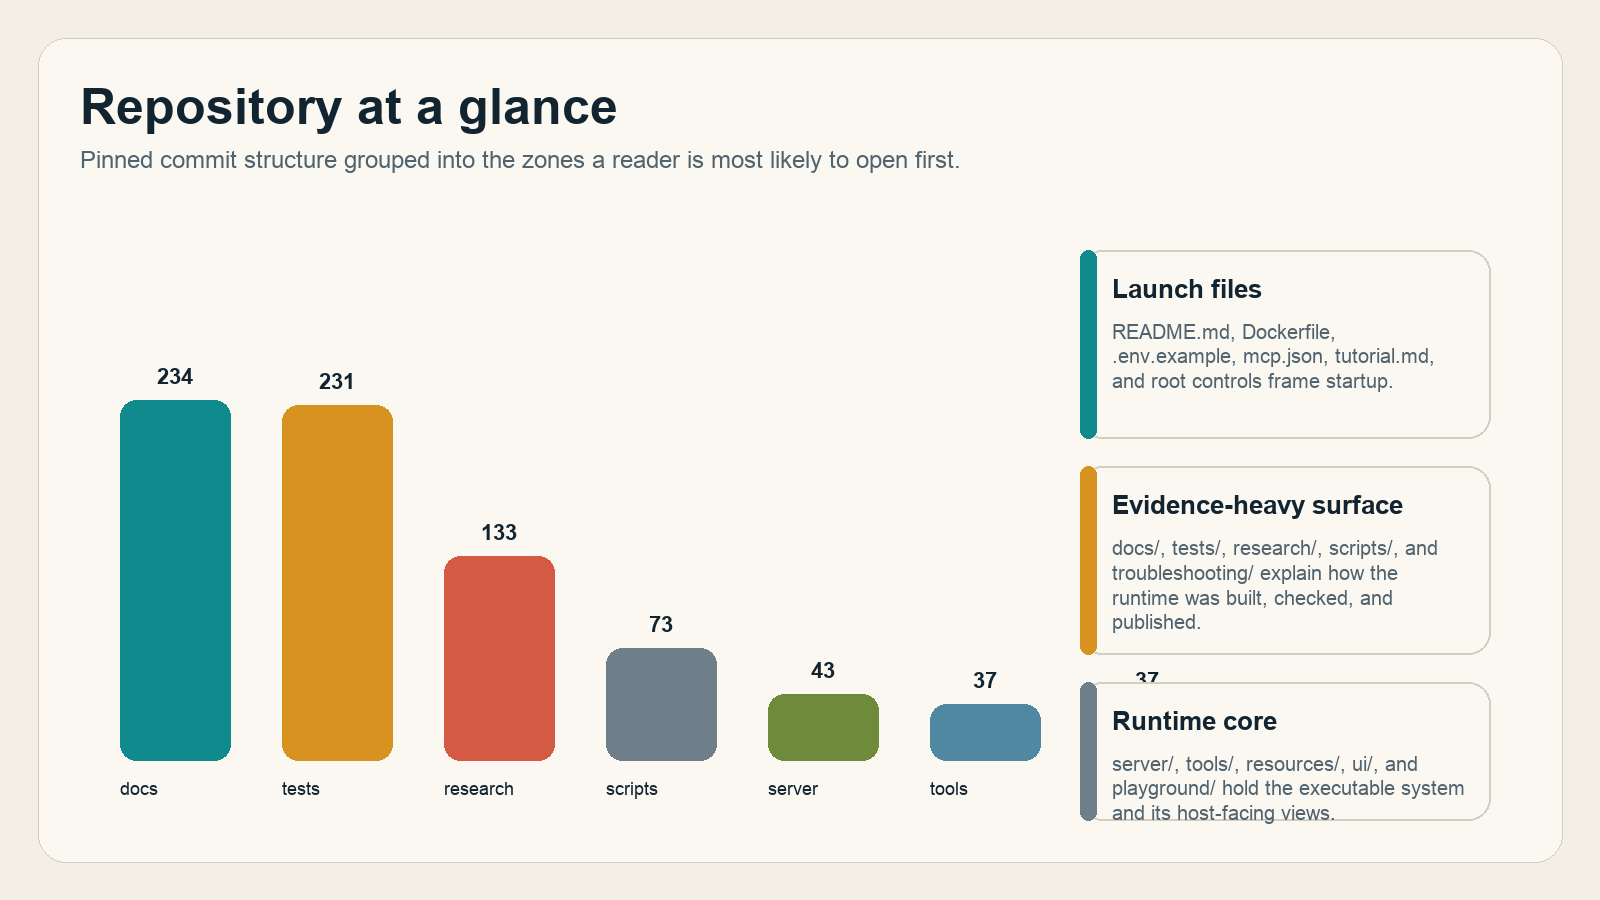
\includegraphics[width=0.96\linewidth,height=\textheight,keepaspectratio,alt={Figure F01. Repository at a glance}]{figures/f01_repo_at_a_glance.png}
\caption{Figure F01. Repository at a glance}
\end{figure}

Figure F01 reduces the pinned commit into one visual: root launch files
up front, runtime code in the middle, and evidence-heavy material
surrounding it.
